
\section*{Introduction}
The goal of this report is to explore the implementation of a queue data structure using a fixed-size array and to discuss the wrap-around technique that helps overcome the limitations typically associated with such an approach. A queue is a fundamental data structure that follows the First-In-First-Out (FIFO) principle, where elements are added at the rear and removed from the front. While queues can be efficiently implemented using linked lists, they require dynamic memory allocation, which may not be optimal in terms of memory usage. On the other hand, an array-based queue can be more efficient in memory utilization, but it faces challenges when elements are removed from the front or when the array becomes full. 


\section*{Method}
The implementation utilized standard C libraries, including \texttt{stdlib.h}, \texttt{stdio.h}, \texttt{time.h}, and \texttt{limits.h}. Measurements were conducted on an Intel i7-13700K CPU with default frequency settings. The code was compiled using GCC without optimizations (\texttt{-O0}). Code from previous labs was used to conduct the benchmark. The benchmark methodology includes random generation of array elements, 50 iterations to obtain reliable average measurements, and time measurements in nanoseconds using \texttt{clock\_gettime()}. Internet tool "mycurvefit.com" have been used to find the best fit function for the data.

\section*{Hypothesis}
The wrap-around technique addresses these challenges by allowing the queue to "wrap around" the array, effectively reusing the space occupied by removed elements. This report will present the implementation of a wrap-around queue, analyze its performance, and compare it with other queue implementations. The hypothesis is that the wrap-around queue will demonstrate improved performance in terms of time complexity compared to a standard array-based queue, particularly when dealing with large numbers of enqueue and dequeue operations. The wrap-around technique should allow for constant-time operations, $O(1)$, regardless of the size of the queue or the number of elements added or removed.

\section*{Inplementation}
\begin{figure}
    \centering
    \includegraphics[width=0.5\textwidth]{IMG_20211006_0001.jpg}
    \caption{Illustration of the logic of the wrap implementation}
    \label{fig:wrap_illustration}
\end{figure}

In this paragraph, some important code snippets will be shown and explained.
To achive the wrap queue, there are many approachs to be done. The figure \ref{fig:wrap_illustration} shows the logic of the wrap implementation. TO achive the goal please follow the following steps:


\subsection*{Code Review}
\subsubsection*{Structure of wrap queue}
\begin{minted}{c}
    typedef struct queue {
        int arraySize;
        int *list;
        int firstIndex;
        int lastIndex;
        int count;        
    } queue;

    queue *create_queue(int arraySize) {
        queue *q = (queue*)malloc(sizeof(queue));
        int *list = (int *)malloc(arraySize * sizeof(int));
        q->arraySize = arraySize;
        q->list = list;
        q->firstIndex = 0;
        q->lastIndex = 0;
        q->count = 0;
        return q;
    }
\end{minted}
The first thing to do is to create a structure for the queue. The structure will contain the size of the array, the array itself, the first index of the queue, the last index of the queue, and the count of the queue. After that we need to create a function to create the queue. The function will create a queue of array with a specific size, and set all the values of the queue to 0. Then the function will return the created queue.
The code above shows an example implementation of the structure of the queue. The time complexity of the create\_queue function is $O(1)$.

\subsubsection*{Enque a number to the queue}
\begin{minted}{c}
    void enque(queue* q, int v) {
        if (q->count == q->arraySize) {
            extendQueue(q);
        }
        
        q->list[q->lastIndex] = v;
        q->lastIndex = (q->lastIndex + 1) % q->arraySize; 
        q->count++;
    }
\end{minted}
The second thing to do is to implement the enque function. The function will add a number to the queue. If the the count number of the queue equals to array size of the queue it means the queue is full, the function will extend the queue. Then the function will add the number to the last index of the queue. The last index of the queue will be updated to the next index of the last index. The time complexity of the enque function is $O(1)$.

\subsubsection*{Extend the queue}
\begin{minted}{c}
    void extendQueue(queue *q) {
        int *biggerList = (int *)malloc(q->arraySize * 2 * sizeof(int));
        
        for (int i = 0; i < q->count; i++) {
            int oldIndex = (q->firstIndex + i) % q->arraySize;
            biggerList[i] = q->list[oldIndex];
        }
        
        free(q->list);
        q->list = biggerList;
        q->firstIndex = 0;  
        q->lastIndex = q->count;  
        q->arraySize = q->arraySize * 2;
    }
\end{minted}
The third thing to do is to implement the extendQueue function. The function will extend the queue by creating a new array with double the size of the old array. The function will copy the elements from the old array to the new array by using a for loop, which will iterate through the old array by start the postion of the first index of the queue and loop till first index of the queue plus the count of the queue, if the index is greater than the array size of the queue, the index will be mod by the array size of the queue. After the elements are migrated, the old array will be freed, and the new array will be assigned to the queue. The first index of the queue will be set to 0, the last index of the queue will be set to the count of the queue, and the array size of the queue will be doubled. The time complexity of the extendQueue function is $O(n)$.


\subsubsection*{dequeue a number from the queue}
\begin{minted}{c}
    int dequeue(queue *q) {
        int res = 0;
        if (q->count > 0) { 
            res = q->list[q->firstIndex];
            q->firstIndex++;
            q->count--;
            if (q->firstIndex >= q->arraySize) {
                q->firstIndex = 0;
            }
        }
        return res;
    }
\end{minted}
The last thing to do is to implement the dequeue function. If the queue is not empty, the function will remove the first element of the queue by increase the first by one, then reduce the queue count by one and return the value of the first element. But there is some corder cases that need to be handled, if the first index of the queue go over the boundary of the array, the first index of the queue will be set to 0. If there is no element in the queue, the function will simply return 0. The time complexity of the dequeue function is $O(1)$.


\section*{Performance and Analysis}
\subsection*{Performance}
\begin{table}[h]
    \centering
    \begin{tabular}{|l|c|c|c|c|}
    \hline
    \textbf{Size} & \textbf{Min (µs)} & \textbf{Max (µs)} & \textbf{Avg (µs)} & \textbf{Avg/op (ns)} \\
    \hline
    1000 & 39.12 & 49.85 & 39.59 & 39.59 \\
    2000 & 20.37 & 88.76 & 23.06 & 11.53 \\
    4000 & 40.57 & 48.46 & 41.14 & 10.28 \\
    8000 & 63.53 & 125.07 & 86.19 & 10.77 \\
    16000 & 135.28 & 326.90 & 159.38 & 9.96 \\
    32000 & 270.83 & 313.61 & 278.27 & 8.70 \\
    64000 & 566.03 & 630.08 & 580.05 & 9.06 \\
    128000 & 1138.72 & 1258.10 & 1181.11 & 9.23 \\
    \hline
    \end{tabular}
    \caption{Performance of Wrap implementation}
    \label{tab:wrap_perf}
\end{table}
From the \ref{tab:wrap_perf} can we see the development of the time complexity of the wrap queue. From the Avg/op column can we tell the time complexity of performing a wrap queue interaction is $O(1)$, which is a constant time complexity. The time complexity of the wrap queue is better than the normal queue implementation, which has a time complexity of $O(n)$. It is also better than improved queue implementation, which has a time complexity of $O(1)$ but the arvage run time per operation lands on 15 nano second instead of 10 nano second.


\subsection*{Analysis}
\begin{figure}[h]
    \centering
    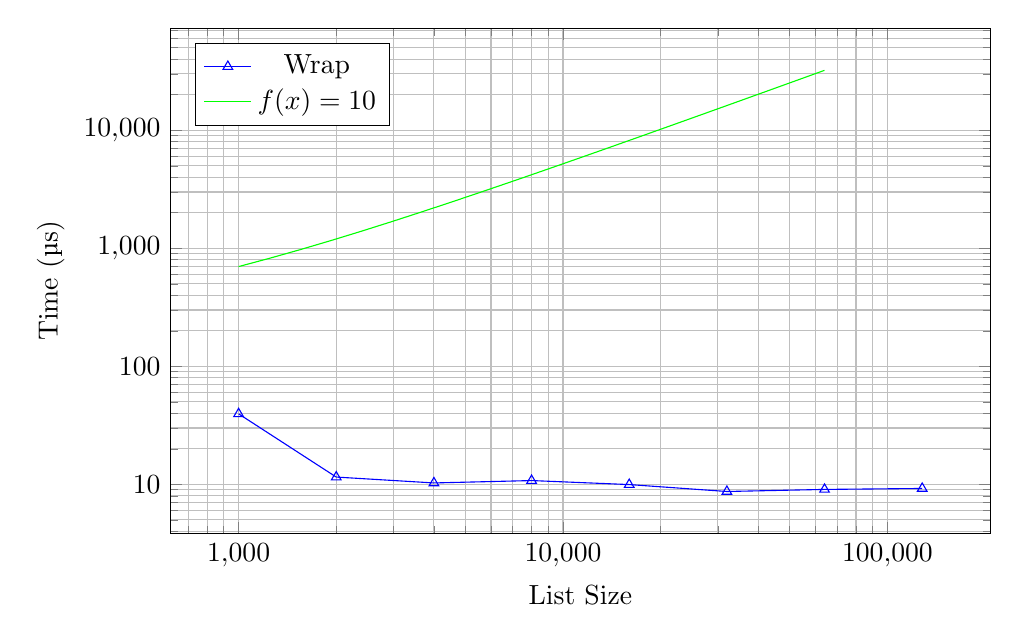
\begin{tikzpicture}
    \begin{axis}[
    xlabel={List Size},
    ylabel={Time (µs)},
    width=12cm,
    height=8cm,
    xmode=log,
    ymode=log,
    grid=both,
    legend pos=north west,
    log ticks with fixed point
    ]
    % Wrap
    \addplot[blue, mark=triangle] coordinates {
    (1000, 39.59)
    (2000, 11.53)
    (4000, 10.28)
    (8000, 10.77)
    (16000, 9.96)
    (32000, 8.70)
    (64000, 9.06)
    (128000, 9.23)
    };
    \addlegendentry{Wrap}

    \addplot[color=green, domain=1000:64000, samples=20] {x/2 + 200};
    \addlegendentry{$f(x) = 10$}
    
    \end{axis}
    \end{tikzpicture}
    \caption{Log-log plot for Wrap queueand the arvage run time per operation for Wrap queue}
    \label{fig:wrap_linked_comparison}
\end{figure}
From \ref{fig:wrap_linked_comparison} can we clearly see the arvage run time per operation for the wrap queue is constant number of 10 nano second per operation.


\section*{Conclusion}
In this report, we have discussed the implementation of a queue using a fixed-size array with a wrap-around technique to efficiently manage memory and avoid unnecessary shifting of elements. The wrap-around solution allows us to maximize the use of the available space in the array by making the front and rear indices circular, ensuring that elements can be added or removed without the need to resize or rearrange the array unless absolutely necessary. This solution significantly improves the efficiency of queue operations by ensuring that both the enqueue and dequeue operations run in constant time, $O(1)$.

One of the key benefits of the wrap-around technique is its ability to utilize memory more effectively than traditional queue implementations, where shifting elements or resizing the array could lead to higher memory overhead and slower performance. Furthermore, the dynamic resizing implemented here ensures that the queue can grow in size as needed, maintaining an efficient balance between space and performance. The time complexity of all main operations remains constant, $O(1)$, which contrasts favorably with other implementations that could exhibit more expensive operations in terms of time and memory.

Overall, this approach demonstrates how careful design choices in data structure implementation, such as the use of wrap-around indexing, can lead to significant improvements in both performance and memory efficiency. This solution can be particularly useful in real-world applications where memory usage is critical and where large numbers of enqueue and dequeue operations need to be performed at high speeds. Moving forward, one potential area for improvement could be the introduction of a more sophisticated resizing strategy that takes into account the rate of queue operations, further enhancing its scalability in high-performance scenarios.

The wrap-around queue serves as a valuable example of dynamic data structures and showcases the importance of understanding trade-offs between performance and complexity in real-world applications. By mastering such techniques, developers can optimize their solutions for better resource utilization, ensuring that their systems remain efficient even under heavy loads.